\newpage
\section*{Appendix A} \label{append:a}
\section*{General}
Link to the Ethics form and Participant Information Sheet:

\url{https://falmouthac-my.sharepoint.com/:f:/g/personal/to231922_falmouth_ac_uk/EiE3vOcxqLlLuU0_BN7m1NoBCja231kbqKHAxOlqX-sRfw?e=4dc65R}
\\
\\
Link to the Computing Artefact GitHub repository: 
\url{https://github.falmouth.ac.uk/TO231922/computing-artefact}
\begin{figure}[ht]
    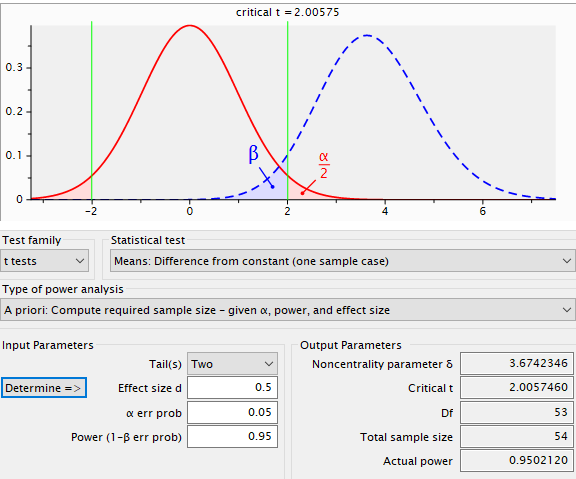
\includegraphics[width=0.48\textwidth]{./Images/gpower.png}
    \centering
    \caption{G*Power Sample Size}
    \label{gpower}
\end{figure}

\newpage
\section*{Appendix B}
\section*{Acknowledgements}
\label{append:b}

\newpage
\section*{Appendix C}
\section*{Reflective Addendum}
\label{append:C}


\newpage
\section*{Appendix D}
\section*{Data Analysis}
\label{append:d}
\begin{lstlisting}[language=R, caption = Example R code for a Two Tailed T-Test using data from an imported CSV file]
    # Load the necessary library to read from CSV files
    library(readr)

    # Load the CSV file
    researchData <- read_csv("D:/R/ArtefactDataAnalysis/research_data.csv")

    # Perform a Two Tailed T-Test
    twoTailed <- t.test(researchData$artefactPicks , researchData$humanPicks)

    # Summarise the results
    summary(twoTailed)
\end{lstlisting}


\newpage
\section*{Appendix E}
\section*{Software Architecture}
\label{append:e}
\begin{figure}[ht]
    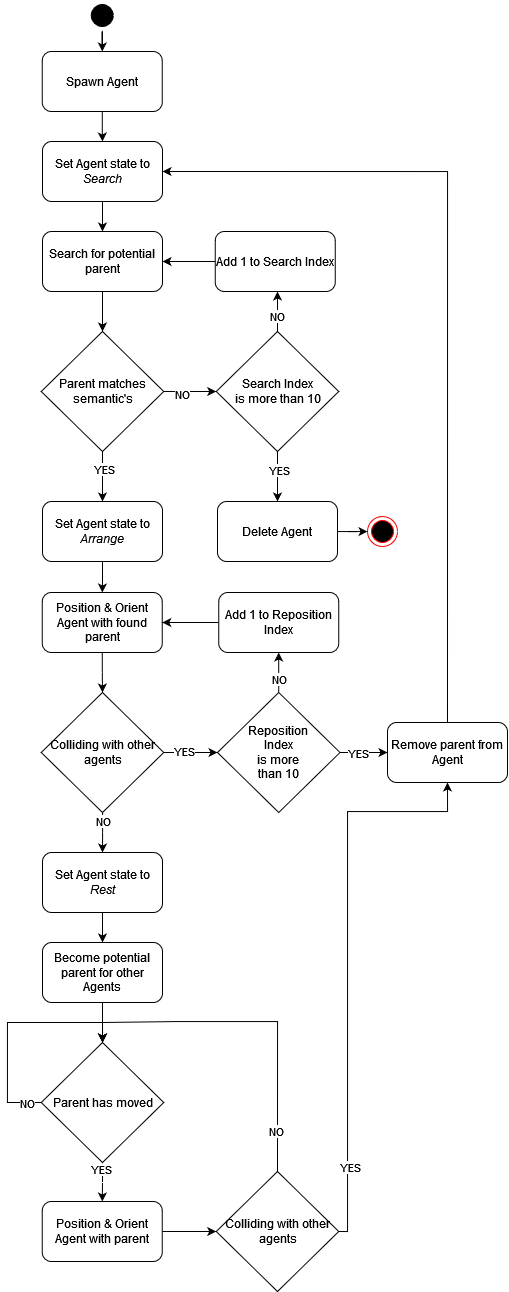
\includegraphics[width=0.45\textwidth]{./Images/AgentActivityDiagram.png}
    \centering
    \caption{Agent Behaviour represented in an Activity Diagram}
    \label{activity-diagram}
\end{figure}

\newpage
\section*{Appendix F}
\section*{Testing}
\label{append:f}
The Unit tests for my artefact were created using Unity's Test Framework and were used throughout the Artefact's development to validate the code and to ensure the Artefact worked as intended. (Unit testing code can be seen in Appendix H).
\\
A small pilot study was conducted with the help of some BSc peers. This pilot study was conducted to ensure the validity of my research methodology. It consisted of them taking part in my 2-staged A/B test, helping in testing the effectiveness of how room interiors were being represented - any feedback received from this small study was implemented into my methodology and no data from this pilot study was used within my data analysis.

\newpage
\section*{Appendix G}
\section*{R Code}
\label{append:g}

\newpage
\section*{Appendix H}
\section*{Unit Testing Code}
\label{append:h}
\lstinputlisting[language=csh, label=UnitTestCode, caption=Unit Test Code used to validate the Artefact's code., captionpos =b]{Code/UnitTesting.cs}